% =============================================================================
% Block 6 --- Aula 6: general equilibrium (Kurlat ch. 9). Checks: practice-all-topics-check-b.py, Block 6.
% Solution format (rules/00_estilo_avaliacao.md §4): Notation list, numbered equations cited with \eqref,
% one operation per displayed line. Labels: b6q<question>:<name>.
\bloco{6}{General equilibrium: two periods, the welfare theorem, infinite horizon}{Kurlat ch.~9 (Aula 6) \,\textbullet\, 25 points}

\questao{(5 points) Objective items.}

\textbf{a)} (3 points) In Kurlat's economy of \S9.1--\S9.2 (price-taking households and firms, a market for every good at every
date), which statement is correct?
\begin{alternativas}
\item Because the competitive equilibrium is Pareto efficient, its steady state must maximize consumption per worker (the golden rule).
\item An equilibrium in which the poorest households consume very little cannot be Pareto efficient, whatever the market structure.
\item If a firm's output imposes a cost on households for which no market exists, the equilibrium can be inefficient with price takers.
\item An unequal equilibrium with capital below the golden rule proves that markets are incomplete, so a planner would save more.
\end{alternativas}
\gabarito{C}
\begin{sol}
\begin{notacao}
\item $F_K$: marginal product of capital; $\delta\in(0,1)$: depreciation rate; $\beta\in(0,1)$: discount factor.
\end{notacao}
\passo{key}{The first welfare theorem needs a price for everything agents care about. A cost imposed outside any market (an
externality, such as pollution from a soy-processing plant) is a missing market: the firm does not pay it, the household cannot
sell the right to impose it, and the equilibrium can be Pareto dominated even though everyone takes prices as given.}
\passo{distractors}{A confuses Pareto efficiency with the golden rule. The efficient steady state satisfies the \emph{modified}
golden rule}
\begin{equation}
F_K-\delta=\frac1\beta-1, \label{b6q16:mgr}
\end{equation}
which has less capital than the golden rule $F_K=\delta$ (Exercise 9.11 in the next question). B confuses efficiency with
equity: an allocation that gives almost everything to one person can be efficient. D makes both mistakes at once: inequality and
capital below the golden rule are each compatible with complete markets and efficiency, by \eqref{b6q16:mgr}.
\refbib{Kurlat (2020), \S9.2 (The First Welfare Theorem), pp.~168--172; Exercise 9.1, p.~179.}
\end{sol}

\medskip
\textbf{b)} (2 points, T or F) In a two-period endowment economy with a representative household, $u=\ln c$ and endowments
$(y_1,y_2)$, news that $y_2$ will be higher raises the equilibrium real interest rate, while consumption in period 1 stays at $y_1$.
\gabarito{T}
\begin{sol}
\begin{notacao}
\item $c_t$, $y_t>0$: consumption and endowment in period $t$; $r$: real rate; $a$: bonds bought in period 1; $\beta\in(0,1)$.
\end{notacao}
\passo{proof}{The Euler equation of the log-utility household is}
\begin{equation}
\frac1{c_1}=\beta(1+r)\frac1{c_2}. \label{b6q16:euler}
\end{equation}
The representative household cannot lend to itself, so the credit market clears at $a=0$:
\begin{equation}
c_1=y_1,\qquad c_2=y_2. \label{b6q16:clear}
\end{equation}
Substituting \eqref{b6q16:clear} into \eqref{b6q16:euler} and solving for $1+r$:
\begin{align}
\frac1{(y_1)}&=\beta(1+r)\frac1{(y_2)}\nonumber\\
1+r^\ast&=\frac{y_2}{\beta y_1}, \label{b6q16:r}
\end{align}
which is increasing in $y_2$. Everyone wants to borrow against the richer future; the rate rises until nobody does, and
$c_1=y_1$ is unchanged by \eqref{b6q16:clear}.
\refbib{Kurlat (2020), \S9.1, pp.~165--168.}
\end{sol}

% -----------------------------------------------------------------------------
\questao{(8 points) \textit{Source: Kurlat, P. (2020), \emph{A Course in Modern Macroeconomics}, Exercise 9.11 ``Patience and
Investment'', p.~185 --- statement reproduced verbatim, all items (a)--(c); item (d) is added by this list.}}

\noindent Suppose the production function is $F(K,L)=K^{\alpha}L^{1-\alpha}$, and the labor supply is exogenous and equal to $L=1$. The
representative household's preferences are given by:
\[
\sum_{t=0}^{\infty}\beta^t\,\frac{c_t^{1-\sigma}}{1-\sigma}
\]
and the depreciation rate is $\delta$.
\begin{enumerate}[label=(\alph*),leftmargin=2.2em,topsep=2pt,itemsep=1pt]
\item Use equation (9.3.17) to find an expression for the level of capital that this economy will have in the steady state.
\item Find an expression for the level of GDP that the economy will have in the steady state.
\item Find an expression for the steady-state investment-to-GDP ratio. How does it depend on $\beta$? Explain.
\end{enumerate}
\noindent\textit{Our note, not in the book:} Kurlat's eq.~(9.3.17) is the steady-state condition of the infinite-period economy;
rearranged on p.~177 it reads $F_K(K_{ss},1)=\frac1\beta-1+\delta$.\par

\noindent\textit{Added parts (not in the book):}\par\nopagebreak
\textbf{d)} (3 of the 8 points) Compare the steady-state investment-to-GDP ratio of (c) with the golden-rule saving rate of the Solow
model with the same technology and depreciation. Which is larger, and why does this not contradict the first welfare theorem?
What happens as $\beta\to1$? Evaluate everything at $\alpha=0.4$, $\beta=0.95$, $\delta=0.08$ (the values of Exercise 9.12).
\resolespaco
\begin{sol}
\begin{notacao}
\item $K_t$: capital (labor is fixed at 1); $Y=F(K,1)=K^\alpha$: output, with capital share $\alpha\in(0,1)$; $F_K$: marginal product.
\item $c_t$: consumption; $I_t$: investment; $\beta\in(0,1)$: discount factor; $\delta\in(0,1)$: depreciation rate.
\item $\sigma>0$: curvature of the period utility in Exercise 9.11 (it does not affect the steady state); $r_{t+1}$: real rate.
\item $X\equiv\frac1\beta-1+\delta>0$: the gross required return net of one (defined in step (a)).
\item $K_{ss}$, $Y_{ss}$: steady-state capital and GDP; $K_{GR}$, $s_{GR}$: golden-rule capital and saving rate.
\end{notacao}
\passo{(a) steady-state capital}{The household's Euler equation is}
\begin{equation}
\left(\frac{c_{t+1}}{c_t}\right)^{\sigma}=\beta(1+r_{t+1}). \label{b6q17:euler}
\end{equation}
In the steady state $c_{t+1}=c_t=c$, so \eqref{b6q17:euler} gives
\begin{align}
\left(\frac{c}{c}\right)^{\sigma}&=\beta(1+r)\nonumber\\
1+r&=\frac1\beta. \label{b6q17:r}
\end{align}
The investment firm's no-arbitrage condition is
\begin{equation}
1+r=F_K-\delta+1. \label{b6q17:arb}
\end{equation}
Equating \eqref{b6q17:r} and \eqref{b6q17:arb} gives Kurlat's eq.~(9.3.17):
\begin{align}
\Big(\frac1\beta\Big)&=F_K(K,1)-\delta+1\nonumber\\
F_K(K,1)-\delta&=\frac1\beta-1. \label{b6q17:mgr}
\end{align}
With $F=K^\alpha$, $F_K=\alpha K^{\alpha-1}$. Substituting into \eqref{b6q17:mgr} and using $X$:
\begin{align}
(\alpha K^{\alpha-1})-\delta&=\frac1\beta-1\nonumber\\
\alpha K^{\alpha-1}&=\frac1\beta-1+\delta\equiv X. \label{b6q17:foc}
\end{align}
Solve \eqref{b6q17:foc} for $K$:
\begin{align}
K^{1-\alpha}&=\frac{\alpha}{X},\nonumber\\
K_{ss}&=\left(\frac{\alpha}{\frac1\beta-1+\delta}\right)^{\frac1{1-\alpha}} \label{b6q17:Kss}\\
&=\left(\frac{\alpha\beta}{1-\beta+\beta\delta}\right)^{\frac1{1-\alpha}}.\nonumber
\end{align}
At the given values:
\begin{align*}
X&=\tfrac1{0.95}-1+0.08=0.0526+0.08=0.1326,\\
\frac{\alpha}{X}&=\frac{0.4}{0.1326}=3.016,\\
K_{ss}&=3.016^{1/0.6}=6.30.
\end{align*}
\passo{(b) GDP}{Evaluate the technology at \eqref{b6q17:Kss}:}
\begin{align}
Y_{ss}&=K_{ss}^\alpha \nonumber\\
&=\left(\left(\frac{\alpha}{\frac1\beta-1+\delta}\right)^{\frac1{1-\alpha}}\right)^{\alpha}\nonumber\\
&=\left(\frac{\alpha}{\frac1\beta-1+\delta}\right)^{\frac{\alpha}{1-\alpha}}. \label{b6q17:Y}
\end{align}
It is increasing in $\beta$: a more patient household requires a lower return on capital, so it accumulates more. Numerically
$Y_{ss}=6.30^{0.4}=2.087$. It does not depend on $\sigma$: in a steady state consumption is flat, so the willingness to substitute
over time never binds.
\passo{(c) investment ratio}{Capital accumulates as}
\begin{equation}
K_{t+1}=(1-\delta)K_t+I_t. \label{b6q17:acc}
\end{equation}
Setting $K_{t+1}=K_t=K$ in \eqref{b6q17:acc}:
\begin{align}
(K)&=(1-\delta)K+I\nonumber\\
I&=\delta K. \label{b6q17:I}
\end{align}
Divide \eqref{b6q17:I} by \eqref{b6q17:Y}, then use $K_{ss}^{1-\alpha}=\alpha/X$ from \eqref{b6q17:Kss}:
\begin{align}
\frac IY&=\frac{\delta K_{ss}}{K_{ss}^\alpha}\nonumber\\
&=\delta K_{ss}^{1-\alpha}\nonumber\\
&=\delta\left(\frac{\alpha}{\frac1\beta-1+\delta}\right)\nonumber\\
&=\frac{\alpha\delta}{\frac1\beta-1+\delta} \label{b6q17:IY}\\
&=\frac{\alpha\beta\delta}{1-\beta+\beta\delta}.\nonumber
\end{align}
Numerically:
\[
\frac IY=\frac{0.4\times0.08}{0.1326}=0.2413 .
\]
By \eqref{b6q17:r}, $X=r+\delta$, so \eqref{b6q17:IY} is the capital share times the depreciation share of the gross return,
$\frac{\delta}{r+\delta}$: investment only replaces worn-out capital.
\passo{(d) golden rule}{Steady-state consumption is output minus the investment \eqref{b6q17:I}:}
\begin{equation}
c=K^\alpha-\delta K. \label{b6q17:cgr}
\end{equation}
Maximize \eqref{b6q17:cgr} over $K$:
\begin{equation}
\alpha K^{\alpha-1}=\delta. \label{b6q17:grfoc}
\end{equation}
Solve \eqref{b6q17:grfoc} for $K$:
\begin{align}
K_{GR}&=\left(\frac\alpha\delta\right)^{\frac1{1-\alpha}}\nonumber\\
&=\left(\frac{0.4}{0.08}\right)^{\frac1{1-0.4}}=5^{1/0.6}=14.62. \label{b6q17:Kgr}
\end{align}
The saving rate that sustains it is $\delta K/Y$, as in \eqref{b6q17:IY}; using \eqref{b6q17:grfoc}, $K_{GR}^{1-\alpha}=\alpha/\delta$:
\begin{align}
s_{GR}&=\delta K_{GR}^{1-\alpha}\nonumber\\
&=\delta\cdot\frac\alpha\delta\nonumber\\
&=\alpha=0.4. \label{b6q17:sgr}
\end{align}
Compare \eqref{b6q17:IY} with \eqref{b6q17:sgr}. Since $\frac1\beta-1>0$, the fraction $\frac{\delta}{\frac1\beta-1+\delta}$ is below 1, so
\[
\frac IY=\alpha\,\frac{\delta}{\frac1\beta-1+\delta}<\alpha=s_{GR}\quad\text{and}\quad K_{ss}=6.30<K_{GR}=14.62 .
\]
No contradiction: the golden rule ranks steady states only and ignores the consumption given up to build the extra capital. An
impatient household values that sacrifice, so the efficient plan stops where the net return equals the rate of time preference,
\eqref{b6q17:mgr} (the modified golden rule), not where $F_K=\delta$ as in \eqref{b6q17:grfoc}. As $\beta\to1$,
$\frac1\beta-1\to0$, so in \eqref{b6q17:IY} $\frac IY\to\alpha$, and \eqref{b6q17:mgr} becomes \eqref{b6q17:grfoc}: $K_{ss}\to K_{GR}$.
\intuicao{Solow fixes $s$ by assumption; here $s$ is the outcome of patience and technology. Equilibrium and golden rule coincide
only for a household that does not discount the future.}
\refbib{Kurlat (2020), \S9.3, eqs.~(9.3.11)--(9.3.17), pp.~172--179, and \S4.3 (golden rule). Same conditions as Lista~5 Q2(c)--(e);
the instructor's key (PSET5, Q2(c)--(d)) derives $1+r_{t+1}=r^K_{t+1}+1-\delta$ and the Euler equation used in (a).}
\rubrica{
\item (a) 2 pts: Euler at $c_{t+1}=c_t$ (1), arbitrage and $K_{ss}$ (1). (b) 1 pt. (c) 2 pts: $I=\delta K$ (1), ratio (1).
\item (d) 3 pts: $s_{GR}=\alpha$ derived (1), comparison (1), why no contradiction and $\beta\to1$ (1).
\item Golden-rule saving with the exponent dropped ($c\propto(1-s)s^{1/(1-\alpha)}$ instead of $s^{\alpha/(1-\alpha)}$): max.\ 1 pt in (d).
\item Saying ``the equilibrium is inefficient because $K_{ss}<K_{GR}$'': max.\ 1 pt in (d). Arithmetic slip with correct method: $-0.5$.
}
\end{sol}

% -----------------------------------------------------------------------------
\questao{(12 points) Discursive. \emph{A frontier economy: from one household's plan to the law of motion of capital.}
A stylized agricultural frontier (think of Brazil's Centro-Oeste) lasts two periods. A representative household has
$\ln c_1+\beta\ln c_2$, $0<\beta<1$, owns the initial capital $K_1>0$, has one unit of time in each period and gets no utility from
leisure. It also owns the representative firm, which rents capital at $R_t$ and labor at $w_t$ and produces
$Y_t=AK_t^{\alpha}L_t^{1-\alpha}$, $0<\alpha<1$. Capital depreciates fully after one period of use ($\delta=1$). In period 1 the household
can buy new capital $K_2$ (one unit of output each) and trade a one-period bond $a_1$ at the real rate $r$.}

\textbf{a)} (3 points) Write both budget constraints, listing every income source, and the present-value constraint. Solve the
firm's problem and find its profit. Derive the household's first-order conditions for \emph{every} choice variable.
\resolespaco
\begin{sol}
\begin{notacao}
\item $c_1,c_2>0$: consumption in periods 1 and 2; $\beta\in(0,1)$: discount factor.
\item $K_1>0$: initial capital; $K_2\ge0$: capital bought in period 1 for period 2; $\delta=1$ (full depreciation).
\item $L_t\in[0,1]$: hours worked in period $t$; $Y_t$: output; $A>0$: productivity; $\alpha\in(0,1)$: capital share.
\item $w_t$, $R_t$: real wage and rental rate of capital; $\Pi_t$: the firm's profit, paid to the household.
\item $a_1$: bonds bought in period 1 (negative = borrowing); $r$: real interest rate between the periods.
\item $\lambda_1,\lambda_2>0$: multipliers on the two budgets; $\nu_t\ge0$: multiplier on $L_t\le1$.
\end{notacao}
\passo{firm}{The technology of the statement is}
\begin{equation}
Y_t=AK_t^{\alpha}L_t^{1-\alpha}. \label{b6q18:Y}
\end{equation}
The firm solves, each period,
\begin{equation}
\max_{K_t,L_t}\ AK_t^\alpha L_t^{1-\alpha}-w_tL_t-R_tK_t. \label{b6q18:firm}
\end{equation}
Differentiating \eqref{b6q18:firm} with respect to $L_t$ and $K_t$:
\begin{align}
w_t&=(1-\alpha)AK_t^\alpha L_t^{-\alpha}, \label{b6q18:w}\\
R_t&=\alpha AK_t^{\alpha-1}L_t^{1-\alpha}. \label{b6q18:R}
\end{align}
Multiply \eqref{b6q18:w} by $L_t$ and \eqref{b6q18:R} by $K_t$, and use \eqref{b6q18:Y}: $w_tL_t=(1-\alpha)Y_t$ and $R_tK_t=\alpha Y_t$. Profit is
\begin{align}
\Pi_t&=Y_t-w_tL_t-R_tK_t\nonumber\\
&=Y_t-\big((1-\alpha)Y_t\big)-\big(\alpha Y_t\big)\nonumber\\
&=0. \label{b6q18:Pi}
\end{align}
Constant returns make factor payments exhaust output, but $\Pi_t$ must still be written in the budget.
\passo{budgets}{Resources equal uses in each period. Capital is used up, so $K_2$ pays $R_2$ and nothing else:}
\begin{align}
c_1+K_2+a_1&=w_1L_1+R_1K_1+\Pi_1, \label{b6q18:bc1}\\
c_2&=w_2L_2+R_2K_2+(1+r)a_1+\Pi_2. \label{b6q18:bc2}
\end{align}
Solve \eqref{b6q18:bc2} for $a_1$:
\[
a_1=\frac{c_2-w_2L_2-R_2K_2-\Pi_2}{1+r}.
\]
Substitute it into \eqref{b6q18:bc1}:
\[
c_1+K_2+\left(\frac{c_2-w_2L_2-R_2K_2-\Pi_2}{1+r}\right)=w_1L_1+R_1K_1+\Pi_1 .
\]
Collect terms:
\begin{align}
c_1+\frac{c_2}{1+r}&=w_1L_1+R_1K_1+\Pi_1+\frac{w_2L_2+\Pi_2}{1+r}\nonumber\\
&\quad+K_2\left(\frac{R_2}{1+r}-1\right). \label{b6q18:pv}
\end{align}
\passo{FOCs}{The choice variables are $c_1,c_2,K_2,a_1,L_1,L_2$, with $L_t\le1$. The Lagrangian uses \eqref{b6q18:bc1}--\eqref{b6q18:bc2}:}
\begin{multline}
\mathcal L=\ln c_1+\beta\ln c_2+\lambda_1\big[w_1L_1+R_1K_1+\Pi_1-c_1-K_2-a_1\big]\\
+\lambda_2\big[w_2L_2+R_2K_2+(1+r)a_1+\Pi_2-c_2\big]+\textstyle\sum_t\nu_t(1-L_t). \label{b6q18:lag}
\end{multline}
Differentiating \eqref{b6q18:lag} with respect to each choice variable:
\begin{align}
c_1:&\quad \frac1{c_1}=\lambda_1, \label{b6q18:fc1}\\
c_2:&\quad \frac\beta{c_2}=\lambda_2, \label{b6q18:fc2}\\
a_1:&\quad \lambda_1=(1+r)\lambda_2, \label{b6q18:fa}\\
K_2:&\quad \lambda_1=R_2\lambda_2, \label{b6q18:fK}\\
L_t:&\quad \lambda_tw_t-\nu_t=0,\qquad \nu_t\ge0,\qquad \nu_t(1-L_t)=0. \label{b6q18:fL}
\end{align}
Dividing \eqref{b6q18:fK} by \eqref{b6q18:fa} gives no arbitrage between bonds and capital, so the last term of \eqref{b6q18:pv} is zero:
\begin{equation}
1+r=R_2. \label{b6q18:noarb}
\end{equation}
By \eqref{b6q18:fL}, $\nu_t=\lambda_tw_t>0$ (positive by \eqref{b6q18:fc1}--\eqref{b6q18:fc2}), so the complementary slackness condition forces
\begin{equation}
L_t=1, \label{b6q18:L}
\end{equation}
a corner: work costs no utility. Substituting \eqref{b6q18:fc1} and \eqref{b6q18:fc2} into \eqref{b6q18:fa} gives the Euler equation:
\begin{align}
\Big(\frac1{c_1}\Big)&=(1+r)\Big(\frac\beta{c_2}\Big)\nonumber\\
c_2&=\beta(1+r)c_1. \label{b6q18:euler}
\end{align}
Substituting \eqref{b6q18:noarb} and \eqref{b6q18:L} into \eqref{b6q18:pv}:
\begin{align}
c_1+\frac{c_2}{1+r}&=w_1(1)+R_1K_1+\Pi_1+\frac{w_2(1)+\Pi_2}{1+r}\nonumber\\
&\quad+K_2\left(\frac{(1+r)}{1+r}-1\right)\nonumber\\
c_1+\frac{c_2}{1+r}&=w_1+R_1K_1+\Pi_1+\frac{w_2+\Pi_2}{1+r}. \label{b6q18:pv1}
\end{align}
\rubrica{\item Firm FOCs and $\Pi=0$ shown: 1 pt. \item Budgets with profits and capital income: 1 pt. \item All six FOCs, with the
labor corner: 1 pt. Missing the $L_t$ condition or the profits: max.\ 2 pts in the item.}
\end{sol}

\textbf{b)} (3 points) Define a competitive equilibrium (allocation, prices, conditions). Use market clearing to find $K_2$, $c_1$,
the equilibrium saving rate $K_2/Y_1$ and $r$. Check $c_1$ against the household's present-value constraint.
\resolespaco
\begin{sol}
\begin{notacao}
\item Symbols as in (a). $W$: the household's lifetime resources, the right side of \eqref{b6q18:pv1} (defined in the check).
\end{notacao}
\passo{definition}{An allocation $\{c_1,c_2,K_2,a_1,L_1,L_2\}$ and prices $\{w_1,w_2,R_1,R_2,r\}$ such that (i) given prices, the household's
choices solve its problem; (ii) given prices, the firm maximizes profit in each period; (iii) markets clear: labor $L_t=1$;
capital (household's $K_t$ = firm's $K_t$); bonds $a_1=0$; and goods}
\begin{align}
c_1+K_2&=Y_1, \label{b6q18:g1}\\
c_2&=Y_2. \label{b6q18:g2}
\end{align}
\passo{solve}{With $L_2=1$, \eqref{b6q18:g2} and \eqref{b6q18:Y} give}
\begin{align}
c_2&=AK_2^\alpha(1)^{1-\alpha}\nonumber\\
&=AK_2^\alpha. \label{b6q18:c2}
\end{align}
By \eqref{b6q18:noarb} and \eqref{b6q18:R} with $L_2=1$:
\begin{align}
1+r&=\alpha AK_2^{\alpha-1}(1)^{1-\alpha}\nonumber\\
&=\alpha AK_2^{\alpha-1}. \label{b6q18:r}
\end{align}
Substitute \eqref{b6q18:c2} and \eqref{b6q18:r} into \eqref{b6q18:euler}:
\[
\big(AK_2^\alpha\big)=\beta\,\big(\alpha AK_2^{\alpha-1}\big)c_1 .
\]
Divide by $AK_2^{\alpha-1}$:
\begin{equation}
K_2=\alpha\beta\,c_1. \label{b6q18:K2c1}
\end{equation}
With $L_1=1$, \eqref{b6q18:g1} and \eqref{b6q18:Y} give
\begin{align}
c_1+K_2&=AK_1^\alpha(1)^{1-\alpha}\nonumber\\
c_1&=AK_1^\alpha-K_2. \label{b6q18:c1g}
\end{align}
Substitute \eqref{b6q18:c1g} into \eqref{b6q18:K2c1} and solve for $K_2$:
\begin{align}
K_2&=\alpha\beta(AK_1^\alpha-K_2)\nonumber\\
(1+\alpha\beta)K_2&=\alpha\beta AK_1^\alpha\nonumber\\
K_2&=\frac{\alpha\beta}{1+\alpha\beta}AK_1^\alpha. \label{b6q18:K2}
\end{align}
Substitute \eqref{b6q18:K2} into \eqref{b6q18:c1g}, then divide \eqref{b6q18:K2} by $Y_1=AK_1^\alpha$:
\begin{align}
c_1&=AK_1^\alpha-\left(\frac{\alpha\beta}{1+\alpha\beta}AK_1^\alpha\right)\nonumber\\
&=\frac{AK_1^\alpha}{1+\alpha\beta}, \label{b6q18:c1}\\
\frac{K_2}{Y_1}&=\frac{\big(\frac{\alpha\beta}{1+\alpha\beta}AK_1^\alpha\big)}{AK_1^\alpha}\nonumber\\
&=\frac{\alpha\beta}{1+\alpha\beta}. \label{b6q18:s}
\end{align}
The interest rate is \eqref{b6q18:r} evaluated at \eqref{b6q18:K2}:
\[
1+r=\alpha A\left(\frac{\alpha\beta}{1+\alpha\beta}AK_1^\alpha\right)^{\alpha-1}.
\]
\passo{check}{With $L_1=1$ and \eqref{b6q18:Pi}, period-1 income is output: $w_1+R_1K_1=Y_1$. Divide \eqref{b6q18:w} by \eqref{b6q18:r} (both at $L_2=1$),
then use \eqref{b6q18:K2}:}
\begin{align}
\frac{w_2}{1+r}&=\frac{(1-\alpha)AK_2^\alpha}{\alpha AK_2^{\alpha-1}}\nonumber\\
&=\frac{1-\alpha}{\alpha}K_2\nonumber\\
&=\frac{1-\alpha}{\alpha}\left(\frac{\alpha\beta}{1+\alpha\beta}Y_1\right)\nonumber\\
&=\frac{(1-\alpha)\beta}{1+\alpha\beta}Y_1. \label{b6q18:hw}
\end{align}
So lifetime resources in \eqref{b6q18:pv1}, with $\Pi_2=0$, are
\begin{align}
W&=Y_1+\frac{(1-\alpha)\beta}{1+\alpha\beta}Y_1\nonumber\\
&=Y_1\,\frac{1+\alpha\beta+\beta-\alpha\beta}{1+\alpha\beta}\nonumber\\
&=\frac{(1+\beta)Y_1}{1+\alpha\beta}. \label{b6q18:W}
\end{align}
Substituting \eqref{b6q18:euler} into \eqref{b6q18:pv1}:
\begin{align*}
c_1+\frac{\big(\beta(1+r)c_1\big)}{1+r}&=W\\
c_1+\beta c_1&=W,
\end{align*}
so log utility spends $\frac1{1+\beta}$ of wealth in period 1.
Using \eqref{b6q18:W}:
\begin{align*}
c_1&=\frac{W}{1+\beta}\\
&=\frac1{1+\beta}\left(\frac{(1+\beta)Y_1}{1+\alpha\beta}\right)\\
&=\frac{Y_1}{1+\alpha\beta},
\end{align*}
the same as \eqref{b6q18:c1}. \checkmark
\intuicao{The saving rate is not $\frac{\beta}{1+\beta}$: the household expects wage income in period 2 (human wealth, \eqref{b6q18:hw}), so it saves less
than a household whose whole income arrives in period 1.}
\rubrica{\item Definition with the three conditions and every market: 1 pt. \item $K_2$, $c_1$, saving rate, $r$: 1.5 pts. \item Check: 0.5 pt.
\item Solving the Euler equation without market clearing (no $K_2$ in terms of $K_1$): max.\ 1 pt.}
\end{sol}

\textbf{c)} (3 points) Solve the planner's problem for this economy and compare with (b). Which theorem have you verified, and
what plays the role of the interest rate in the planner's problem?
\resolespaco
\begin{sol}
\begin{notacao}
\item Symbols as in (a); $V(K_2)$: the planner's objective after substituting the constraints; $F_K$: marginal product of capital;
$u'(c)=1/c$.
\end{notacao}
\passo{planner}{The planner maximizes $\ln c_1+\beta\ln c_2$ subject to the resource constraints (labor is 1: it costs nothing)}
\begin{align}
c_1+K_2&=AK_1^\alpha, \label{b6q18:p1}\\
c_2&=AK_2^\alpha. \label{b6q18:p2}
\end{align}
Substituting \eqref{b6q18:p1}--\eqref{b6q18:p2} into the objective:
\begin{align}
V(K_2)&=\ln(AK_1^\alpha-K_2)+\beta\ln\big(AK_2^\alpha\big)\nonumber\\
&=\ln(AK_1^\alpha-K_2)+\beta\ln A+\alpha\beta\ln K_2. \label{b6q18:V}
\end{align}
Differentiate \eqref{b6q18:V} and set it to zero:
\begin{equation}
\frac{1}{AK_1^\alpha-K_2}=\frac{\alpha\beta}{K_2}. \label{b6q18:pfoc}
\end{equation}
Cross-multiplying, \eqref{b6q18:pfoc} is $K_2=\alpha\beta(AK_1^\alpha-K_2)$, the first line of the derivation of \eqref{b6q18:K2}, so
\[
K_2=\frac{\alpha\beta}{1+\alpha\beta}AK_1^\alpha .
\]
The second derivative of \eqref{b6q18:V} is $-\frac1{(AK_1^\alpha-K_2)^2}-\frac{\alpha\beta}{K_2^2}<0$: strictly concave, so this is the maximum.
Same allocation as \eqref{b6q18:K2}--\eqref{b6q18:c1}.
\passo{reading}{The first welfare theorem: the competitive allocation is Pareto efficient (with one household, it is the planner's
optimum). Since $\beta u'(c_2)F_K(K_2)=\frac{\beta\,\alpha AK_2^{\alpha-1}}{AK_2^\alpha}=\frac{\alpha\beta}{K_2}$, \eqref{b6q18:pfoc} reads}
\begin{equation}
u'(c_1)=\beta u'(c_2)F_K(K_2). \label{b6q18:pmrt}
\end{equation}
In the market, \eqref{b6q18:R} and \eqref{b6q18:noarb} give $F_K(K_2)=R_2=1+r$, which turns \eqref{b6q18:pmrt} into the Euler equation
\eqref{b6q18:euler}. The interest rate is the marginal rate of transformation between the two dates, the price that makes the
household's trade-off equal the technology's.
\rubrica{\item Planner's FOC and solution: 1.5 pts. \item Theorem named and $1+r=F_K$ as the MRT: 1.5 pts.}
\end{sol}

\textbf{d)} (3 points) Now let the economy last forever: $\sum_t\beta^t\ln c_t$, same technology, $\delta=1$, $L_t=1$. Show that the rule
$K_{t+1}=\alpha\beta AK_t^\alpha$, $c_t=(1-\alpha\beta)AK_t^\alpha$ satisfies the Euler equation at every date and the transversality condition.
Draw the map $K_{t+1}(K_t)$ with the 45-degree line, find the steady state and its stability, and relate the result to Solow
($\delta=1$, $n=0$) and to the golden rule.
\resolespaco
\begin{sol}
\begin{notacao}
\item $K_t$, $c_t$: capital and consumption at date $t=0,1,\dots$; $A$, $\alpha$, $\beta$ as in (a); $L_t=1$, $\delta=1$.
\item $K^\ast$: steady-state capital of the rule; $s$: Solow's saving rate; $K_{GR}$, $s_{GR}$: golden-rule capital and saving rate.
\end{notacao}
\passo{Euler}{With $\delta=1$ the gross return on capital is $F_K=\alpha AK_{t+1}^{\alpha-1}$, so the Euler equation is}
\begin{equation}
\frac1{c_t}=\beta\,\frac{\alpha AK_{t+1}^{\alpha-1}}{c_{t+1}}. \label{b6q18:eulinf}
\end{equation}
The proposed rule, from the statement:
\begin{align}
K_{t+1}&=\alpha\beta AK_t^\alpha, \label{b6q18:rK}\\
c_t&=(1-\alpha\beta)AK_t^\alpha. \label{b6q18:rc}
\end{align}
Substitute \eqref{b6q18:rc} at $t+1$ into the right side of \eqref{b6q18:eulinf}, then \eqref{b6q18:rK}, then \eqref{b6q18:rc} at $t$:
\begin{align*}
\beta\,\frac{\alpha AK_{t+1}^{\alpha-1}}{(1-\alpha\beta)AK_{t+1}^\alpha}&=\frac{\alpha\beta}{(1-\alpha\beta)K_{t+1}}\\
&=\frac{\alpha\beta}{(1-\alpha\beta)\,\big(\alpha\beta AK_t^\alpha\big)}\\
&=\frac1{(1-\alpha\beta)AK_t^\alpha}=\frac1{c_t}.\qquad\checkmark
\end{align*}
\passo{transversality}{Using \eqref{b6q18:rK} and \eqref{b6q18:rc}, with $u'(c_t)=1/c_t$:}
\begin{align*}
\beta^tu'(c_t)K_{t+1}&=\beta^t\,\frac{1}{\big((1-\alpha\beta)AK_t^\alpha\big)}\,\big(\alpha\beta AK_t^\alpha\big)\\
&=\beta^t\frac{\alpha\beta AK_t^\alpha}{(1-\alpha\beta)AK_t^\alpha}\\
&=\beta^t\frac{\alpha\beta}{1-\alpha\beta}\to0 .\qquad\checkmark
\end{align*}
\passo{steady state}{Set $K_{t+1}=K_t=K^\ast$ in \eqref{b6q18:rK}:}
\begin{align}
K^\ast&=\alpha\beta A{K^\ast}^\alpha\nonumber\\
{K^\ast}^{1-\alpha}&=\alpha\beta A\nonumber\\
K^\ast&=(\alpha\beta A)^{\frac1{1-\alpha}}. \label{b6q18:Kstar}
\end{align}
The map \eqref{b6q18:rK} is concave and starts at 0 with infinite slope. Its slope is $\alpha\cdot\alpha\beta AK_t^{\alpha-1}$; by \eqref{b6q18:Kstar},
$\alpha\beta A{K^\ast}^{\alpha-1}=1$, so the slope at $K^\ast$ is $\alpha<1$: the map crosses the 45-degree line once from above, and $K^\ast$ is stable.
\begin{center}
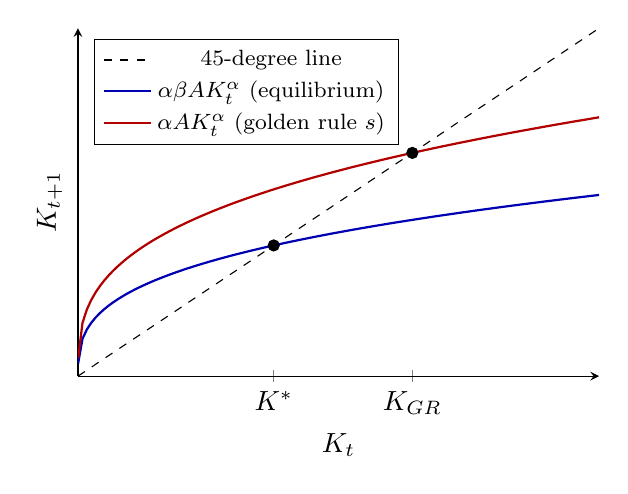
\begin{tikzpicture}
\begin{axis}[width=8.2cm,height=6cm,xmin=0,xmax=0.3,ymin=0,ymax=0.3,xlabel={$K_t$},ylabel={$K_{t+1}$},
  axis lines=left,xtick={0.1127,0.1925},xticklabels={$K^\ast$,$K_{GR}$},ytick=\empty,legend pos=north west,
  legend style={font=\footnotesize}]
\addplot[black,dashed,domain=0:0.3] {x}; \addlegendentry{45-degree line}
\addplot[blue!70!black,thick,domain=0.0001:0.3,samples=120] {(0.7/3)*x^(1/3)}; \addlegendentry{$\alpha\beta AK_t^\alpha$ (equilibrium)}
\addplot[red!70!black,thick,domain=0.0001:0.3,samples=120] {(1/3)*x^(1/3)}; \addlegendentry{$\alpha AK_t^\alpha$ (golden rule $s$)}
\addplot[only marks,mark=*] coordinates {(0.1127,0.1127) (0.1925,0.1925)};
\end{axis}
\end{tikzpicture}\\[-2pt]
{\footnotesize Drawn with $A=1$, $\alpha=1/3$, $\beta=0.7$: $K^\ast=(0.7/3)^{1.5}=0.113$, $K_{GR}=(1/3)^{1.5}=0.192$.}
\end{center}
\passo{Solow}{Solow with $\delta=1$, $n=0$ reads}
\begin{equation}
K_{t+1}=sAK_t^\alpha, \label{b6q18:solow}
\end{equation}
which is \eqref{b6q18:rK} with $s=\alpha\beta$. The difference is that $s$ is \emph{chosen}, from patience and the capital share.
\passo{golden rule}{In a steady state of \eqref{b6q18:solow}, consumption is output minus replacement:}
\begin{equation}
c=AK^\alpha-K. \label{b6q18:cGR}
\end{equation}
Maximize \eqref{b6q18:cGR} over $K$:
\begin{equation}
\alpha AK^{\alpha-1}=1. \label{b6q18:GRfoc}
\end{equation}
The saving rate that sustains it follows from \eqref{b6q18:solow} with $K_{t+1}=K_t$, then \eqref{b6q18:GRfoc}:
\begin{align*}
s_{GR}&=\frac{K}{AK^\alpha}=\frac{1}{AK^{\alpha-1}}\\
&=\frac{1}{(1/\alpha)}\\
&=\alpha>\alpha\beta .
\end{align*}
So $K^\ast<K_{GR}$. At $K^\ast$, \eqref{b6q18:Kstar} gives $\alpha A{K^\ast}^{\alpha-1}=\frac1\beta$: the modified golden rule
$F_K-\delta=\frac1\beta-1$ with $\delta=1$, not \eqref{b6q18:GRfoc}. The two-period economy of (b) saved $\frac{\alpha\beta}{1+\alpha\beta}<\alpha\beta$
\eqref{b6q18:s}: with a last period, capital has no use after it.
\intuicao{One household's Euler equation plus market clearing ($K_{t+1}$ = what it saves) is a Solow law of motion with an
endogenous saving rate. Efficiency (item (c)) and the golden rule answer different questions.}
\refbib{Kurlat (2020), \S9.3, pp.~172--179; \S4.3 (golden rule); Exercise 9.12, p.~185; Prova~01, Q2(e)--(f).}
\rubrica{
\item Euler verified line by line (1), transversality (0.5): 1.5 pts. \item Graph: axes labeled, map, 45-degree line, $K^\ast$ (0.5); stability (0.5).
\item Solow with $s=\alpha\beta$ chosen vs $s_{GR}=\alpha$: 0.5 pt. ``Equilibrium = golden rule'': 0 for this line. No graph: max.\ 2 pts.
}
\end{sol}
